\section{2020 年 12 月 22 日答疑记录}

本次答疑记录是 12 月数学月考里选择、填空题的错题讲解, 原先为两次答疑的内容. 为了方便起见, 所有题均改成解答题, 并整合成一次记录. 

\begin{example}
    已知函数 $f(x)=2-\dfrac3x$, 若 $g(x)= f(x)-m$ 为奇函数, 求实数 $m$ 的值.
\end{example}
\begin{solution}
    方法一: 由题意, $g(x)=2-\dfrac3x-m$ 且 $g(-x)= -g(x)$, 所以
    \[2-\dfrac3{-x}-m= -\biggl(2-\dfrac3x-m\biggl),\quad
        \text{整理得}\quad m=2.\]
    
    方法二: 因为 $f(x)=2-\dfrac3x$ 的图形可由 $y=-\dfrac3x$ 的图形向上平移两个单位长度得到, 而后者关于原点对称 (函数为奇函数), 而 $g(x)= f(x)-m$ 的图形可由 $f(x)$ 的图形上、下平移得到, 所以只需 $m=2$, 即将 $f(x)$ 的图形向下平移两个单位长度, 可得 $g(x)=-\dfrac3x$ 为奇函数.
\end{solution}

\begin{example}
    ``$\ln a>\ln b$'' 是 ``$3^a>3^b$'' 的什么条件?
\end{example}
\begin{solution}
    有 $y=\ln x$ 的定义域为 $(0,+\infty)$ 且单调递增, 可知 $\ln a>\ln b$ 表明 $a>b>0$. 再由 $y=3^x$ 的定义域为 $\realnum$ 且单调递增, 可知 $3^a>3^b$ 表明 $a>b$. 因此 ``$\ln a>\ln b$'' 是 ``$3^a>3^b$'' 的必要不充分条件.
\end{solution}


\begin{example}
    根据有关资料, 围棋状态空间复杂度的上限 $M$ 约为 $3^{361}$, 而可观测宇宙中普通物质的原子总数 $N$ 约为 $10^{80}$. 将 $\dfrac{M}{N}$ 表示为 $10$ 的正整数次方 ($\lg 3\approx 0.48$).
\end{example}
\begin{solution}
    根据对数的运算性质, 
    \[\begin{aligned}
        \lg \dfrac{M}{N}
        &= \lg M-\lg N= \lg 3^{361}- \lg 10^{80}
         = 361\lg 3- 80\\
        &\approx 361\cdot 0.48- 80
         = 93.28,
       \end{aligned}\]
    所以 $\dfrac{M}{N}\approx 10^{93}$.
\end{solution}

\begin{example}
    画出函数 $y= \dfrac{x a^x}{|x|}$ ($0<a<1$) 的图形的大致形状.
\end{example}
\begin{solution}
    利用绝对值的定义, 原函数化为 $y= \begin{cases}
        -a^x, & x<0,\\
        a^x, & x>0,
    \end{cases}$
    图形的大致形状如下:
    
    \begin{center}
        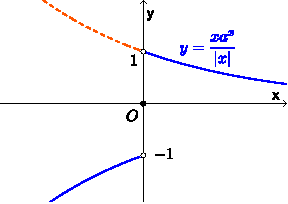
\includegraphics[scale=1.1]{2020-1227-1100-crop}
    \end{center}
\end{solution}


\begin{example}\label{exa:201227-1450}
    求关于 $x$ 的方程 $x=\log_a (-x^2 +2x+a)$ ($a>0$, 且 $a\neq 1$) 的解的个数.
\end{example}
\begin{solution}
    因为 $x=\log_a a^x$, 所以原方程化为
    \[\log_a a^x=\log_a (-x^2 +2x+a),\quad\text{即}\quad
        a^x= -(x-1)^2 +1+a,\]
    故应考虑函数 $f(x)=a^x$ 与 $g(x)= -(x-1)^2 +1+a$ 的图形的交点个数. 分 $0<a<1$ 和 $a>1$ 两种情况画图如下:
    
    \begin{center}
        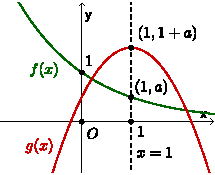
\includegraphics[scale=1.1]{2020-1227-1200-crop}\qquad
        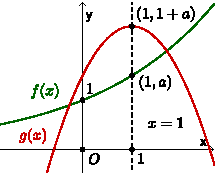
\includegraphics[scale=1.1]{2020-1227-1210-crop}
    \end{center}
    
    由图可知, $f(x)=a^x$ 与 $g(x)= -(x-1)^2 +1+a$ 的图形总有两个交点, 所以方程 $x=\log_a (-x^2 +2x+a)$ 的解的个数为 $2$.
\end{solution}

例~\ref{exa:201227-1450} 也可以直接画原方程 $x=\log_a (-x^2 +2x+a)$ 对应的两个函数 $y=x$ 和 $y=\log_a (-x^2 +2x+a)$ 的大致图形, 画后者之前需适当讨论, 略微麻烦一点.

\begin{example}
    若 $a>b$, 则下列不等式中哪些一定成立?
    
    (1) $\log_2 a> \log_2 b$;\quad 
    (2) $2^a> 2^b$;\quad 
    (3) $a^{\frac13}> b^{\frac13}$;\quad
    (4) $\dfrac1a<\dfrac1b$.
\end{example}
\begin{solution}
    此题主要考查函数的定义域和单调性.
    
    (1) 因为函数 $y=\log_2 x$ 的定义域为 $(0,+\infty)$ 且单调递增, 所以 $\log_2 a> \log_2 b$ 等价于 $a>b>0$, 与已知条件 $a>b$ 不符.
    
    (2) 因为函数 $y= 2^x$ 的定义域为 $\realnum$ 且单调递增, 所以 $2^a> 2^b$ 等价于 $a>b$, 与已知条件 $a>b$ 相同.
    
    (3) 因为函数 $y= x^{\frac13}$ 的定义域为 $\realnum$ 且单调递增, 所以 $a^{\frac13}> b^{\frac13}$ 等价于 $a>b$, 与已知条件 $a>b$ 相同.
    
    (4) 函数 $y=\dfrac1x$ 的定义域为 $(-\infty,0)\cup(0,+\infty)$, 所以 $\dfrac1a<\dfrac1b$ 不一定有意义 (如当 $a=0$ 或 $b=0$ 时). 即使该式有意义, 在已知条件 $a>b$ 中取 $a>0$, $b<0$ 可知 $\dfrac1a>0>\dfrac1b$, 与本小题结论不符.
\end{solution}


\begin{example}
    下列各式中哪些是正确的?
    
    (1) $\sin\dfrac\pi5> \sin\dfrac{6\pi}5$;\quad 
    (2) $\cos\biggl(-\dfrac\pi3\biggr)< \cos\dfrac\pi6$;
    
    (3) $\tan\dfrac\pi4> \tan\dfrac{5\pi}4$;\quad 
    (4) $\sin\dfrac\pi3> \sin\dfrac\pi6$.
\end{example}
\begin{solution}
    画正弦线、余弦线如下:
    
    \begin{center}
        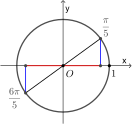
\includegraphics[scale=1.1]{2020-1227-1300-crop}\qquad
        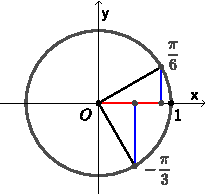
\includegraphics[scale=1.1]{2020-1227-1310-crop}\\[5pt]
        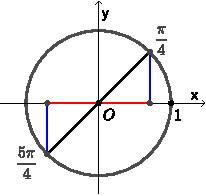
\includegraphics[scale=1.1]{2020-1227-1320-crop}\qquad
        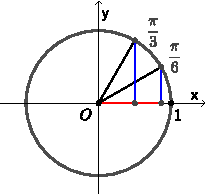
\includegraphics[scale=1.1]{2020-1227-1330-crop}
    \end{center}
    
    由此可知 (正切值由正弦值比余弦值得到)
    \[\begin{gathered}
        \sin\dfrac\pi5>0> \sin\dfrac{6\pi}5,\quad 
        \cos\biggl(-\dfrac\pi3\biggr)=\frac12< \frac{\sqrt3}2=\cos\dfrac\pi6,\\
        \tan\dfrac\pi4= 1= \tan\dfrac{5\pi}4,\quad 
        \sin\dfrac\pi3= \frac{\sqrt{3}}2> \frac12=\sin\dfrac\pi6.
    \end{gathered}\]
\end{solution}

\begin{example}\label{exa:201227-1440}
    已知 $f(x)$ 是定义在 $\realnum$ 上的偶函数, 且当 $x\in(-\infty,0]$ 时, $f(x)=2^x+\dfrac13$, 求 $f\biggl(\log_2 \dfrac32\biggr)$ 的值.
\end{example}
\begin{solution}
    因为 $\log_2 \frac32>\log_2 1=0$, 所以由偶函数的特征,
    \[f\biggl(\log_2 \frac32\biggr)= f(-x)
        = 2^{-\log_2 \frac32}+\frac13
        = 2^{\log_2 \frac23}+\frac13
        = \frac23+\frac13= 1.\]
\end{solution}

例~\ref{exa:201227-1440} 中也可以先求 $f(x)$ 在 $x\in(0,+\infty)$ 时的解析式, 可参考 ``2020 年 11 月 14 日答疑记录'' 的第五个例子和 ``2020 年 11 月 22 日答疑记录'' 的第二个例子. 

\begin{example}
    已知函数 $f(x) =\begin{cases}
        3^x, & x\leqslant 0,\\
        -2x+1, & x>0,
    \end{cases}$ 若 $f(x)\leqslant \dfrac13$, 求实数 $x$ 的取值范围.
\end{example}
\begin{solution}
    (1) 若 $x\leqslant 0$, 则 $f(x)\leqslant \dfrac13$ 化为
    \[3^x\leqslant \frac13= 3^{-1},\quad\text{解得}\quad
        x\leqslant -1.\]
    
    (2) 若 $x> 0$, 则 $f(x)\leqslant \dfrac13$ 化为
    \[-2x+1\leqslant \frac13,\quad\text{解得}\quad
        x\geqslant \frac13.\]
        
    综上所述, $x\in (-\infty,-1]\cup \biggl[\dfrac13,+\infty\biggr)$.
\end{solution}

分段函数分段考虑, 下题也是如此.

\begin{example}
    已知函数 $f(x)= \begin{cases}
        ax+2-3a, & x<0,\\
        2^x-1, & x\geqslant 0.
    \end{cases}$ 若存在 $x_1$, $x_2\in\realnum$, $x_1\neq x_2$, 使得 $f(x_2)= f(x_2)$ 成立, 求实数 $a$ 的取值范围.
\end{example}
\begin{solution}
    题中 $f(x)$ 的图形在 $x<0$ 的部分为半直线, 在 $x\geqslant 0$ 的部分为 $y=2^x$ 向下平移一个单位长度. 而条件 ``存在 $x_1\neq x_2$ 使得 $f(x_2)= f(x_2)$ 成立'' 表明存在水平的直线与 $f(x)$ 的图形有两个不同的交点. 分 $a<0$, $a=0$ 和 $a>0$ 三种情况 (分别对应半直线不同的增减性) 画图如下:
    
    \begin{center}
        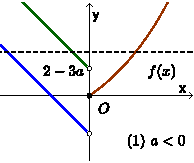
\includegraphics[scale=1.1]{2020-1227-1400-crop}\qquad
        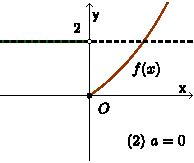
\includegraphics[scale=1.1]{2020-1227-1410-crop}\qquad
        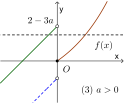
\includegraphics[scale=1.1]{2020-1227-1420-crop}
    \end{center}
    
    由图可知, 当 $a\leqslant 0$ 时, 图形均合题意; 而当 $a>0$ 时, 需 $2-3a>0$ 即 $a<\dfrac23$. 由此可知, 实数 $a$ 的取值范围为 $\biggl(-\infty,-\dfrac23\biggr)$.
\end{solution}